%
%	WISS 2015サンプルファイル (未来ビジョンテンプレート, 最後数行空き問題解決バージョン)
%
%	2010/07/12 Ver 1.0 秋田 純一
%	2010/08/04 Ver 1.1 後藤 真孝
% 	2011/09/27  Ver 1.4 渡邊 恵太 (協力:五十嵐悠紀)
% 	2015/02/08  Ver 1.5 大槻 麻衣
% 	2016/05/26  Ver 1.6 大槻 麻衣


\documentclass[a4paper,twoside,papersize]{wiss}

\usepackage{ascmac}
\usepackage[dvips]{graphicx}
\usepackage{nidanfloat} %% appended in WISS2010 for Future Vision (2010/7/7:akita)
\usepackage{multicol}
%\usepackage{color,array}
%\usepackage{boxedminipage}

%% balance.styを追加 (2012/9/27:watanabe, Igarashi)
\usepackage{balance}    %% 最後のページの高さを揃えるために追加  (2012/9/27:watanabe, Igarashi)
%%% 最後のページの2段組の高さを揃える.\balanceを入れる.
%%% そろえたくないときは,\nobalance

%% urlのOverflow対策
\usepackage{url}

\journalhead{わかるらんど: IoT時代の情報共有視覚化} %%%%%% ←← 著者において必ず記入すること

\begin{document}

\title{わかるらんど: IoT時代の情報共有視覚化}
\etitle{}%2012年では英文タイトルは廃止されました.記入しないでください.
%
%注意
%
%
% WISS2016かラシングルブラインドとなりました.投稿時に氏名と所属を記入してください.
\author{山田 尚昭\affil{慶應義塾大学大学院 政策・メディア研究科}  増井 俊之\affil{慶應義塾大学 環境情報学部}}

\begin{abstract}
人や環境の状態がリアルタイムにわかる視覚化システム「わかるらんど」を提案する.
単一の画面にタイル状に情報を並べて表示するダッシュボードは複数のフロー情報をひと目でチェックするのに効果的な視覚化手法である.
しかし,人間の感情や現在の状況もフロー情報であるが,それらをアウトプットにはSNSが用いられダッシュボードに表示することは今まで行われてこなかった.
これはSNSに投稿される長いテキストメッセージはダッシュボードに表示するには適さないからである.
わかるらんどは人間の感情や現在の状況を,近年のメッセンジャーアプリで利用されているスタンプで表現することで,
ダッシュボードにリアルタイムに人間の感情や現在の状況を表示することを可能にした.
わかるらんどはありとあらゆる場所におけるサイネージや会議やコンファレンスでのチャットシステムとして極めて汎用的な利用が期待できる.
\end{abstract}

\maketitle

\section{はじめに}

WebやIoT機器などから発信されるフロー情報が巷にはあふれている。
フロー情報とはニュースや天気予報、SNSなどリアルタイムに常に流れていく情報のことである。
フロー情報のひとつである「人間の感情や現在の状況」というものをアウトプットする場としてSNSが多くの人に利用されているが、
SNSのタイムラインは投稿したものが流れていってしまったり投稿数の多い人ばかりが目立ってしまったりするという欠点がある。

フロー情報を視覚化する手法としてダッシュボードがある。
ダッシュボードとは単一の画面に情報を並べて表示するもので、センサの値や株価などのフロー情報をひと目で把握するのに非常に便利である。
ダッシュボードには様々な製品やサービスが存在し、多くの組織で利用されている。
ダッシュボードにいろいろな人や環境の状態がリアルタイムに簡単に伝えられ、ひと目で把握できる視覚化システム「わかるらんど」を提案する。
わかるらんどはありとあらゆるフロー情報を非常に簡単に表示できるダッシュボードである。
\section{わかるらんど}

\subsection{ユーザインタフェース}

図\ref{dashboard}図\ref{console}はわかるらんどのスクリーンショットである。
ユーザインタフェースは、ダッシュボード、投稿画面の2つからなる。
ダッシュボードと投稿画面はいずれも単一の画面で、上部のボタンで切り替えて利用する。
ダッシュボードには指定した情報を表示するウィジェット(図\ref{widget})を格子状に並べることができる。

ウィジェットには人間の感情や状態を表示するwakariウィジェットとセンサ情報などの数値を表示するdataウィジェットの2種類がある。
ウィジェットのバックグラウンドには人/物/現象の画像を表示し、その上に情報をオーバーレイで表示する。
情報はリアルタイムに更新が反映され、最新の情報のみを表示する。
投稿画面ではユーザとしてダッシュボードに投稿を行うことができる。
投稿はスタンプをクリックすることで行う。
スタンプはテキストから作ることもできるし画像URLから追加することもできる。
また、スタンプ投稿時にクリックの長さを変えることでダッシュボードに表示する時間を変更することができる。

\begin{figure}
\centering
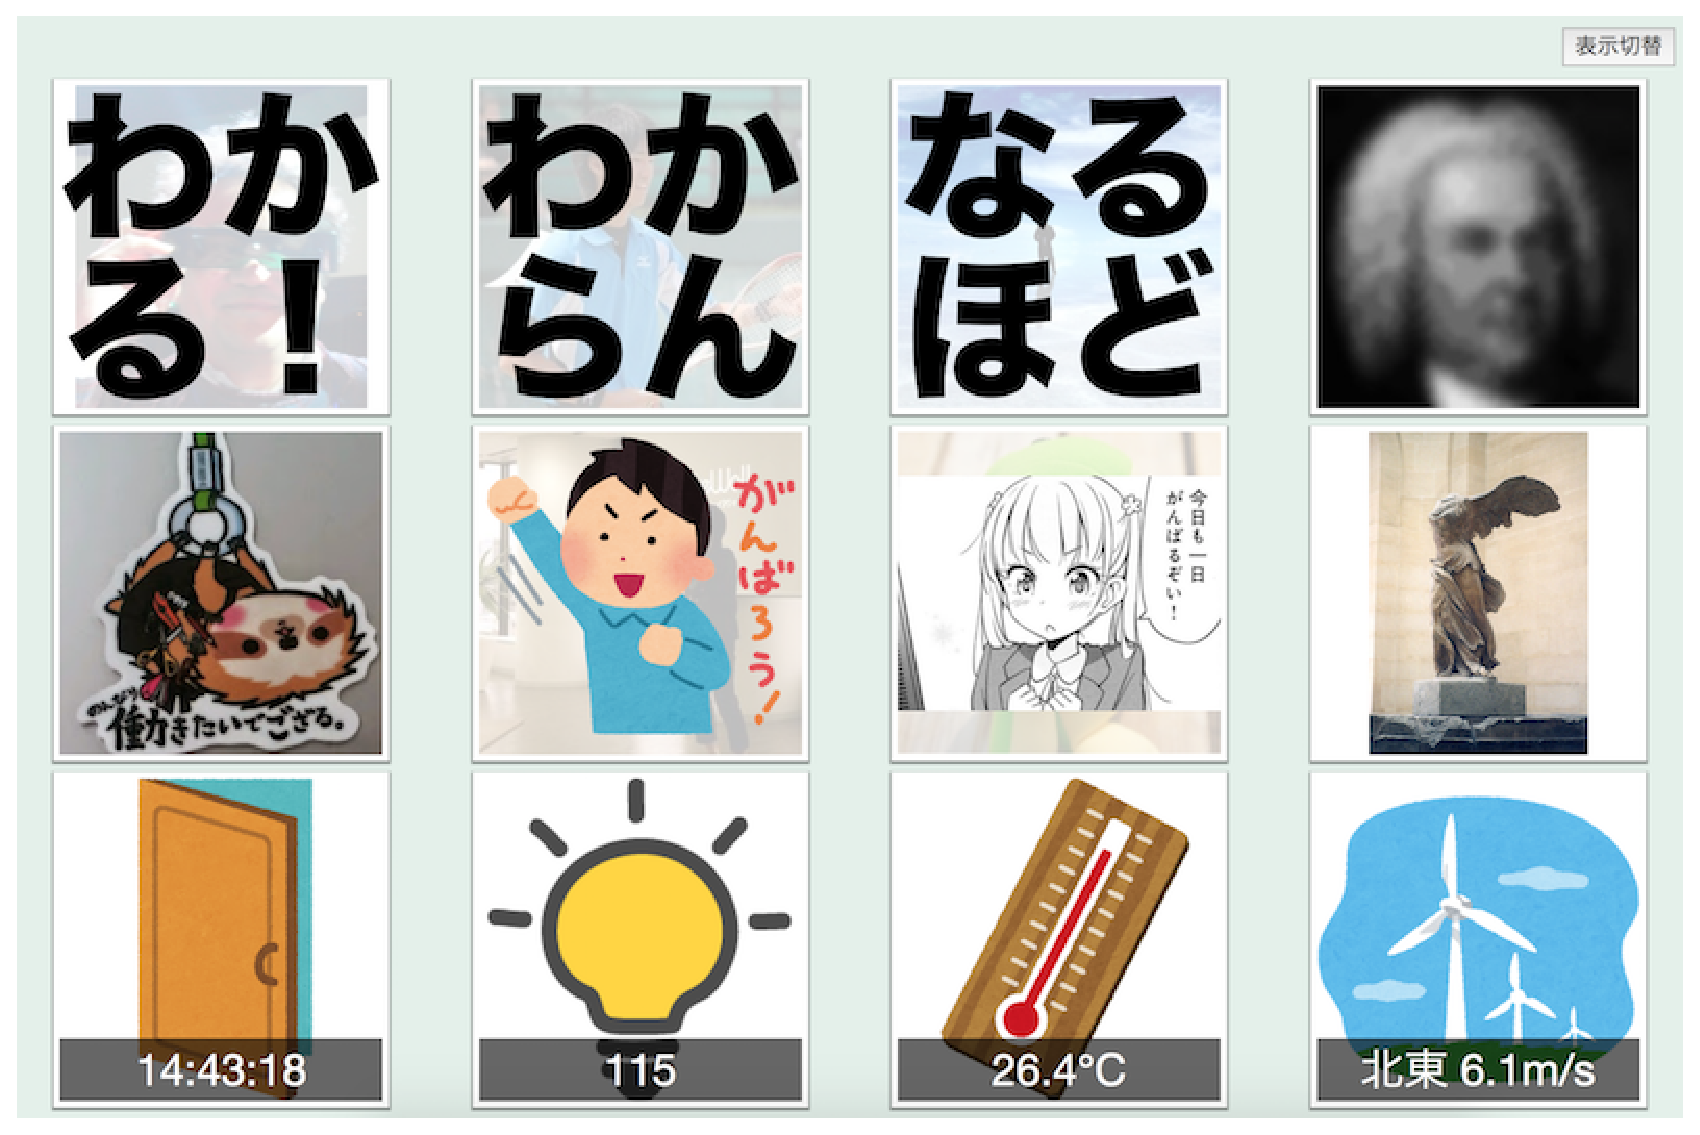
\includegraphics[width=7cm]{images/dashboard.eps}
\caption{ダッシュボード}
\label{dashboard}
\end{figure}

\begin{figure}
\centering
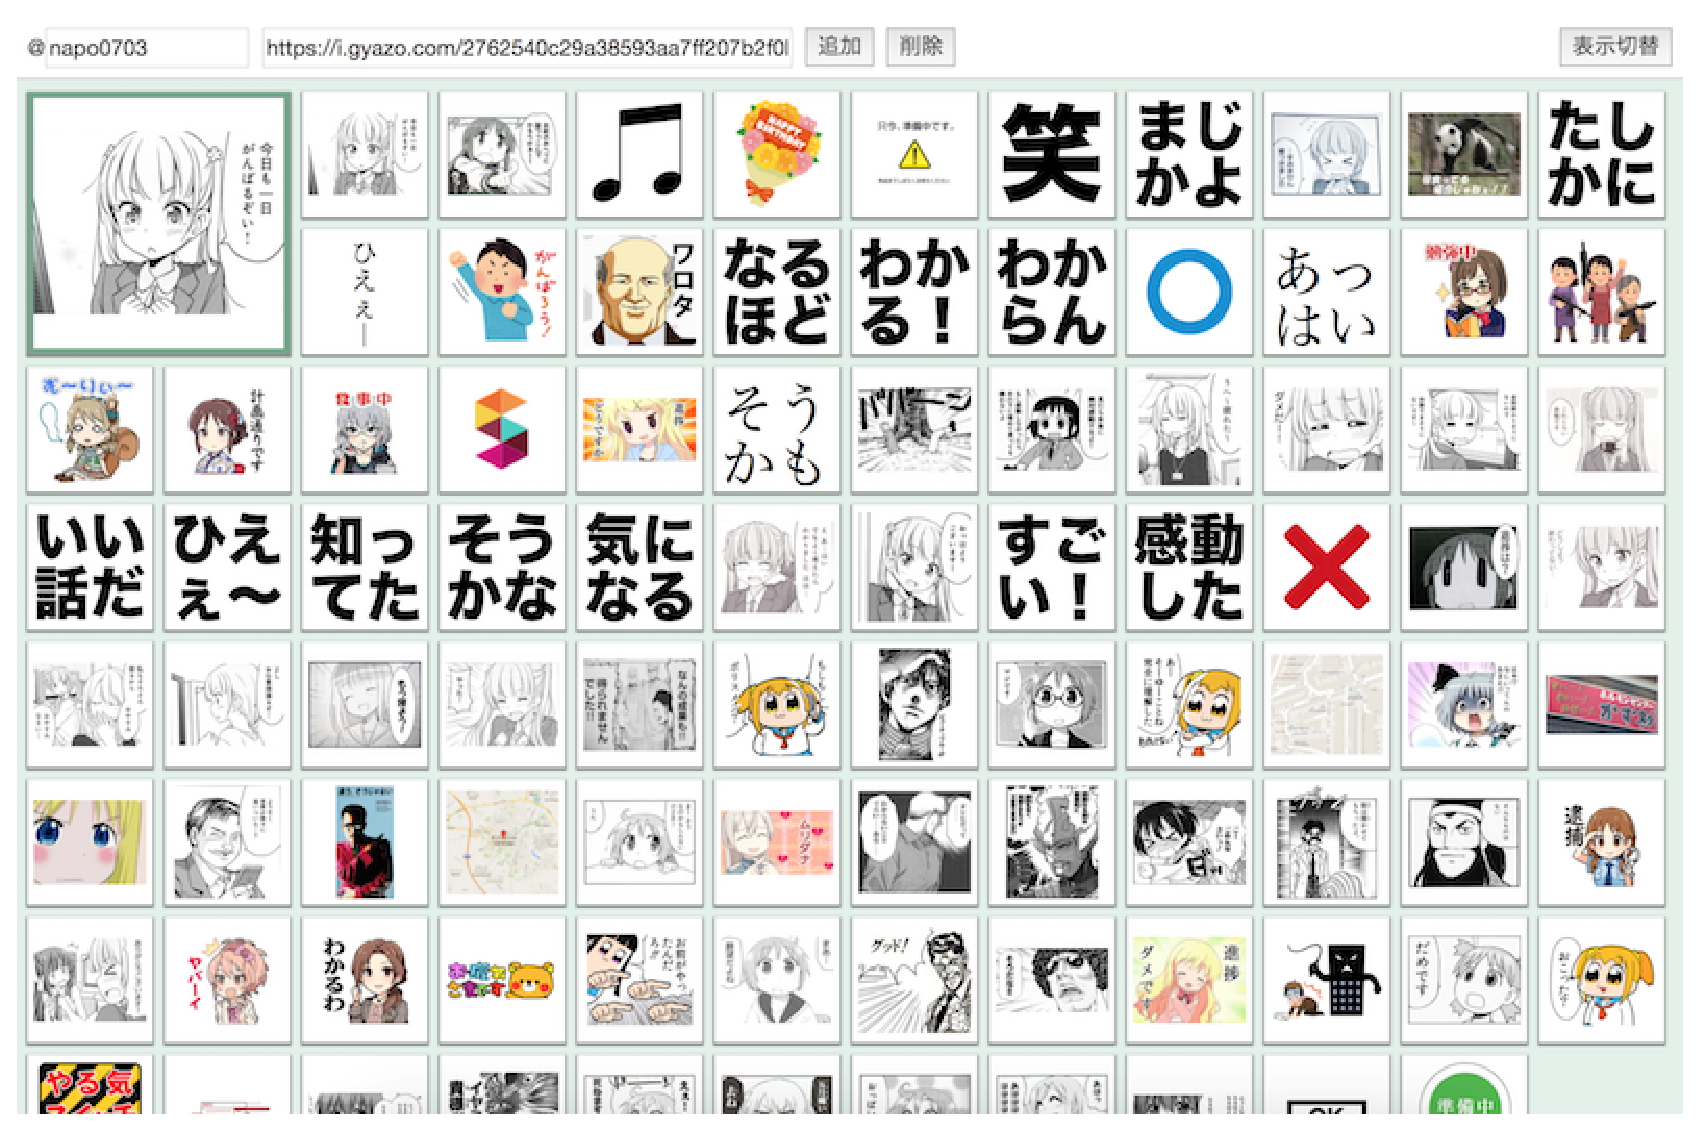
\includegraphics[width=7cm]{images/console.eps}
\caption{投稿画面}
\label{console}
\end{figure}

\begin{figure}
\centering
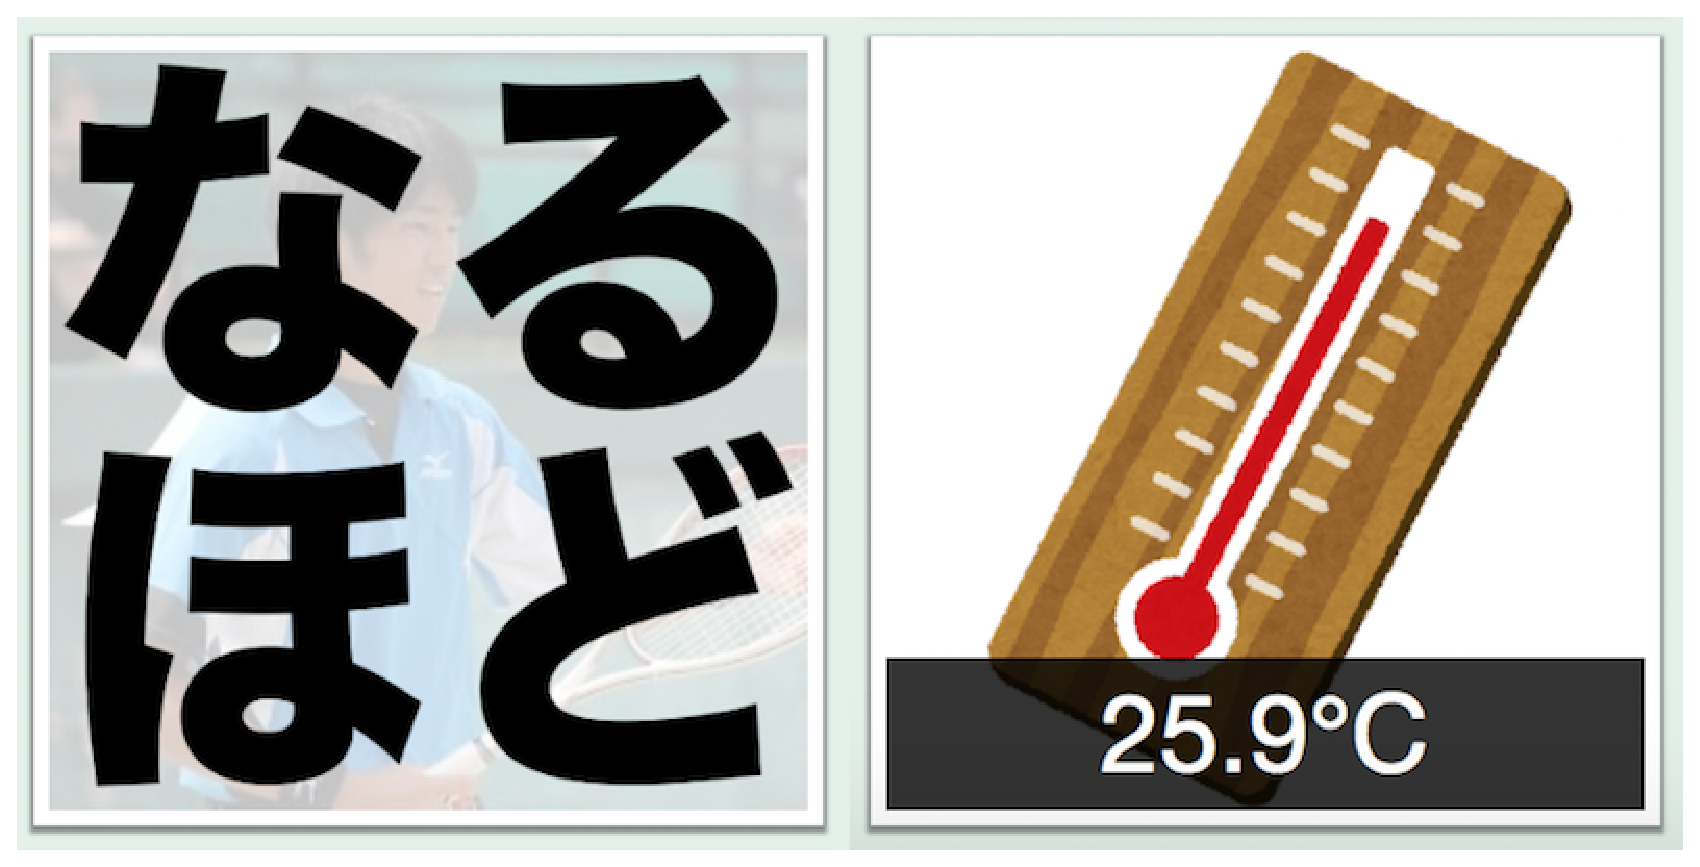
\includegraphics[width=7cm]{images/widget.eps}
\caption{wakariウィジェット(左)とdataウィジェット(右)}
\label{widget}
\end{figure}

\subsection{利用例}

\subsubsection{発表や講義での利用例}

図\ref{discussion}は講義や発表での利用例である。
これをサブスクリーンに表示することで、他の参加者の感情を把握したり登壇者が聴衆の反応を見ながら発表をすることができる。
また図\ref{vote}のようにアンケートを取ったり、図\ref{rescue}のように「寒い」「トイレに行きたい」など、
口頭では伝えにくい感情を周囲に伝えることもできる。

\begin{figure}[h]
\centering
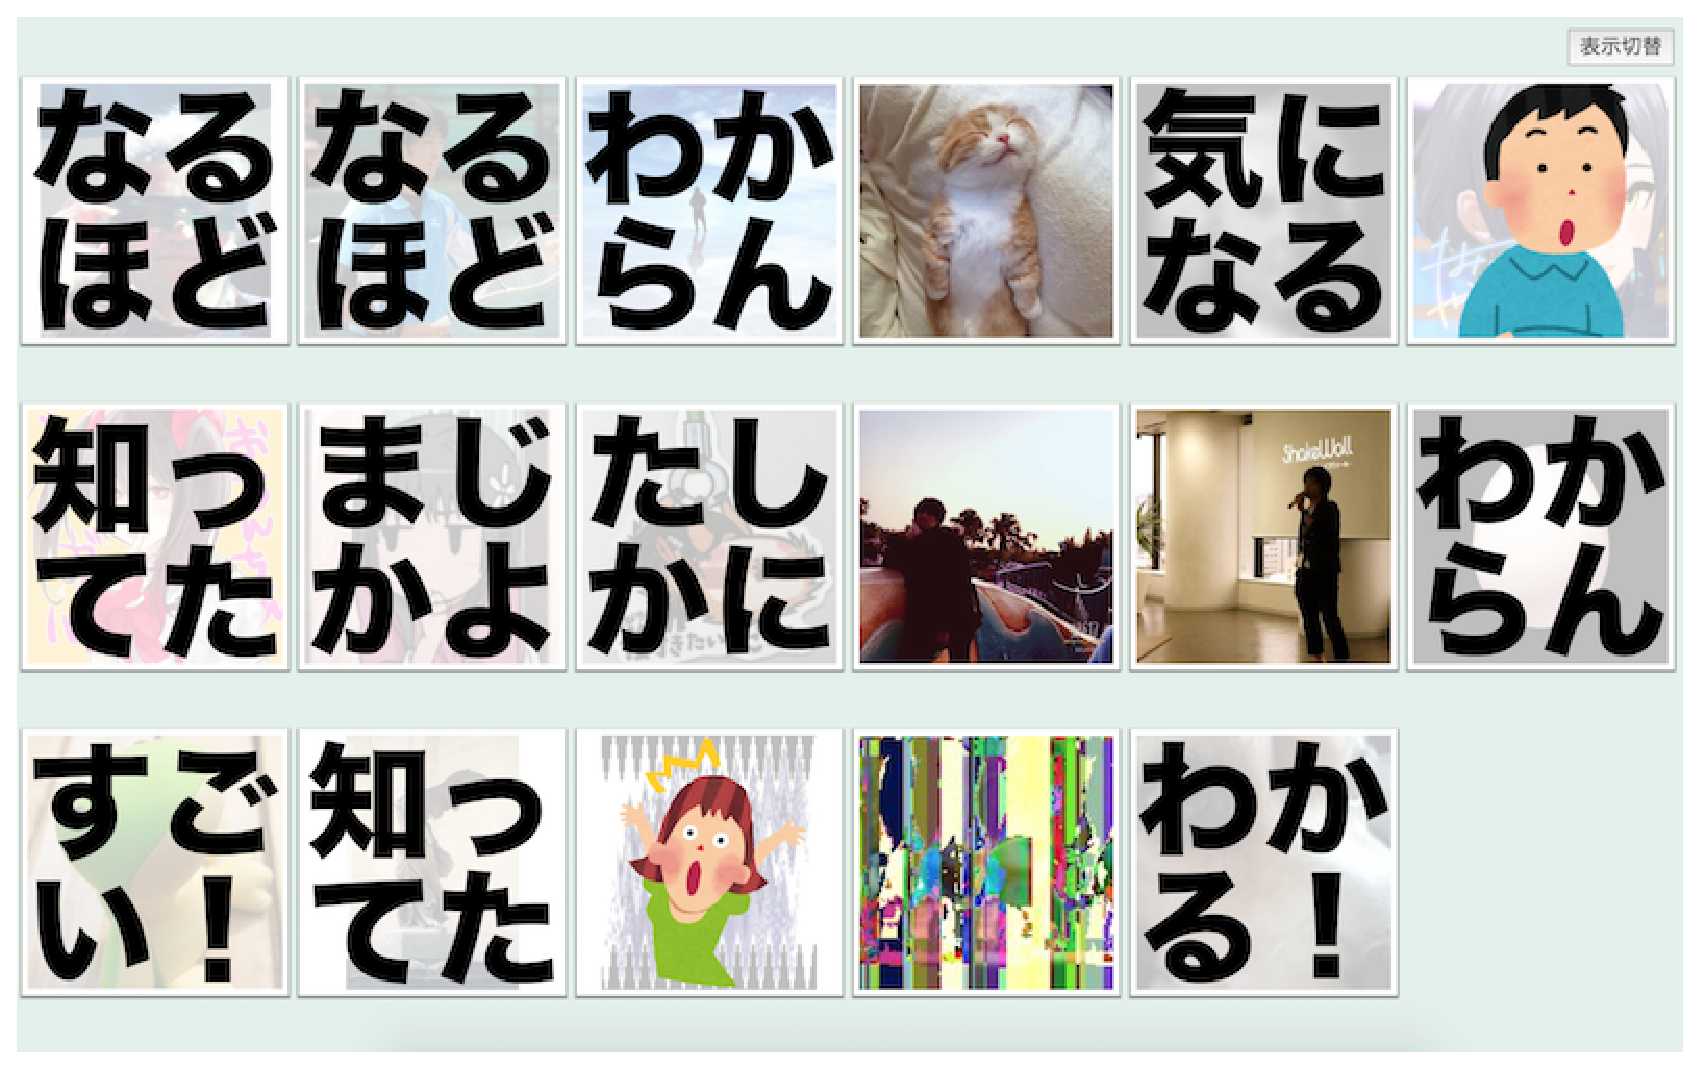
\includegraphics[width=7cm]{images/discussion.eps}
\caption{会議での利用}
\label{discussion}
\end{figure}

\begin{figure}[h]
\centering
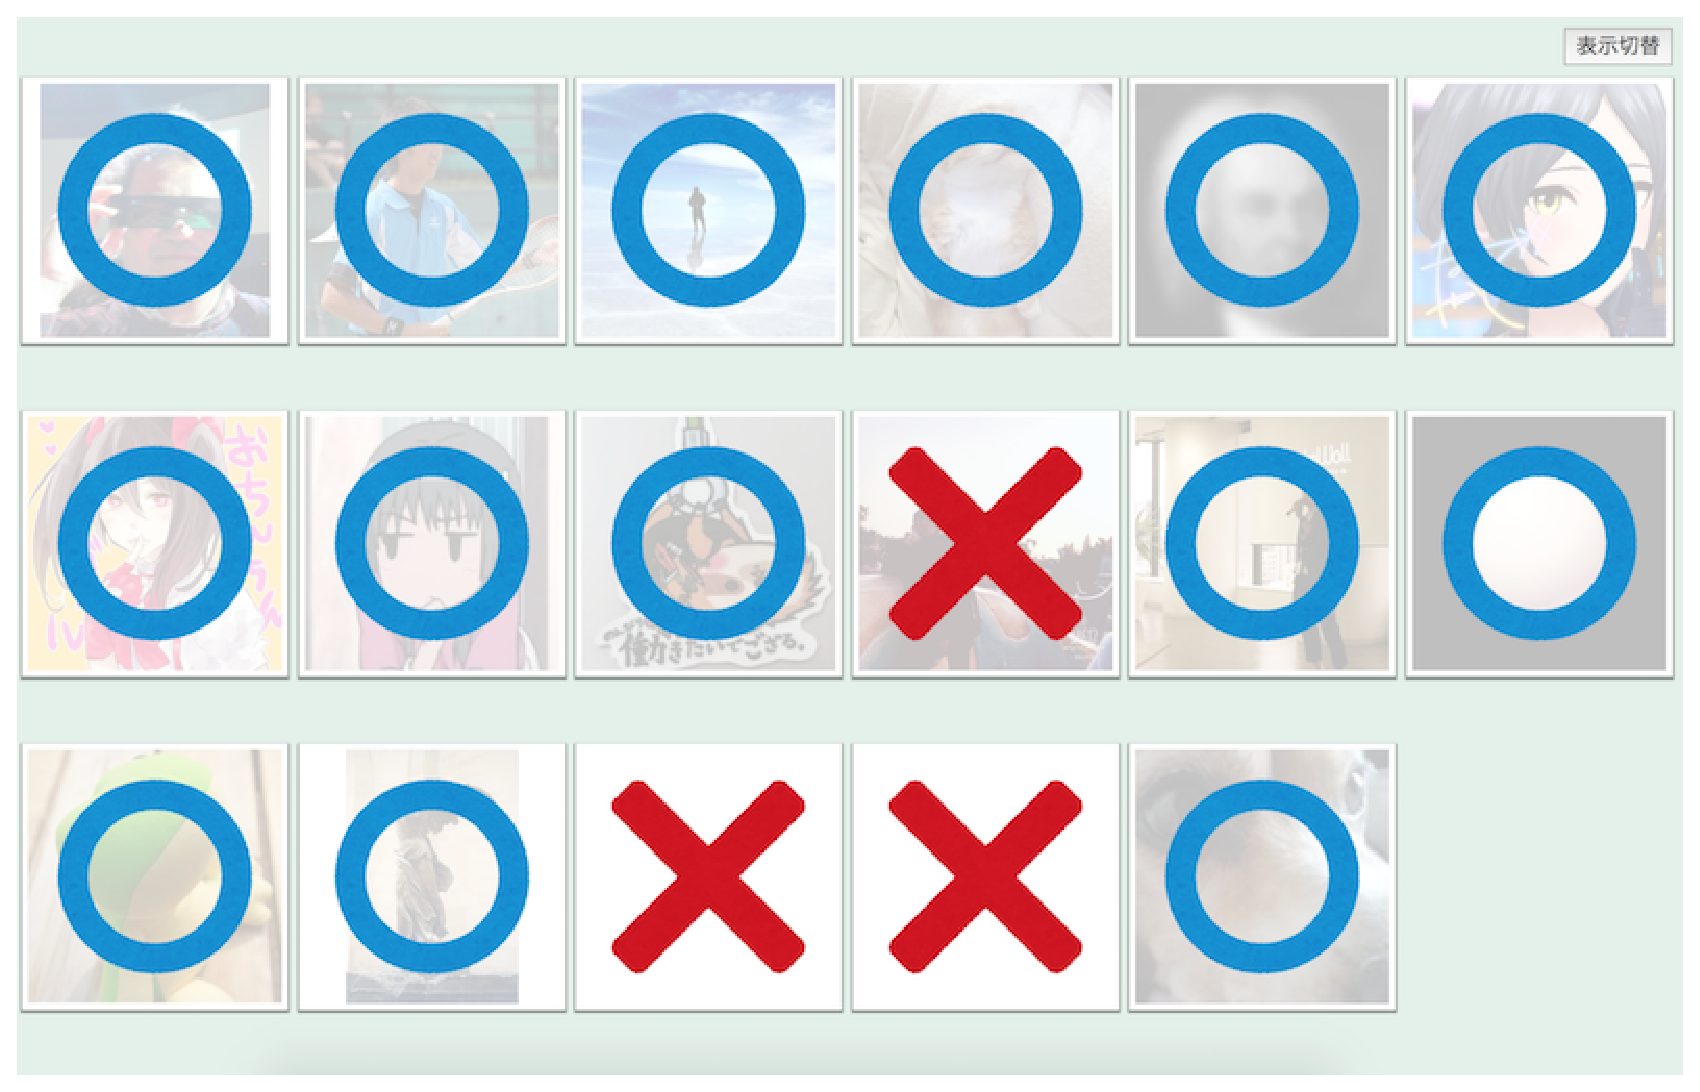
\includegraphics[width=7cm]{images/vote.eps}
\caption{アンケートとしての利用}
\label{vote}
\end{figure}

\begin{figure}[h]
\centering
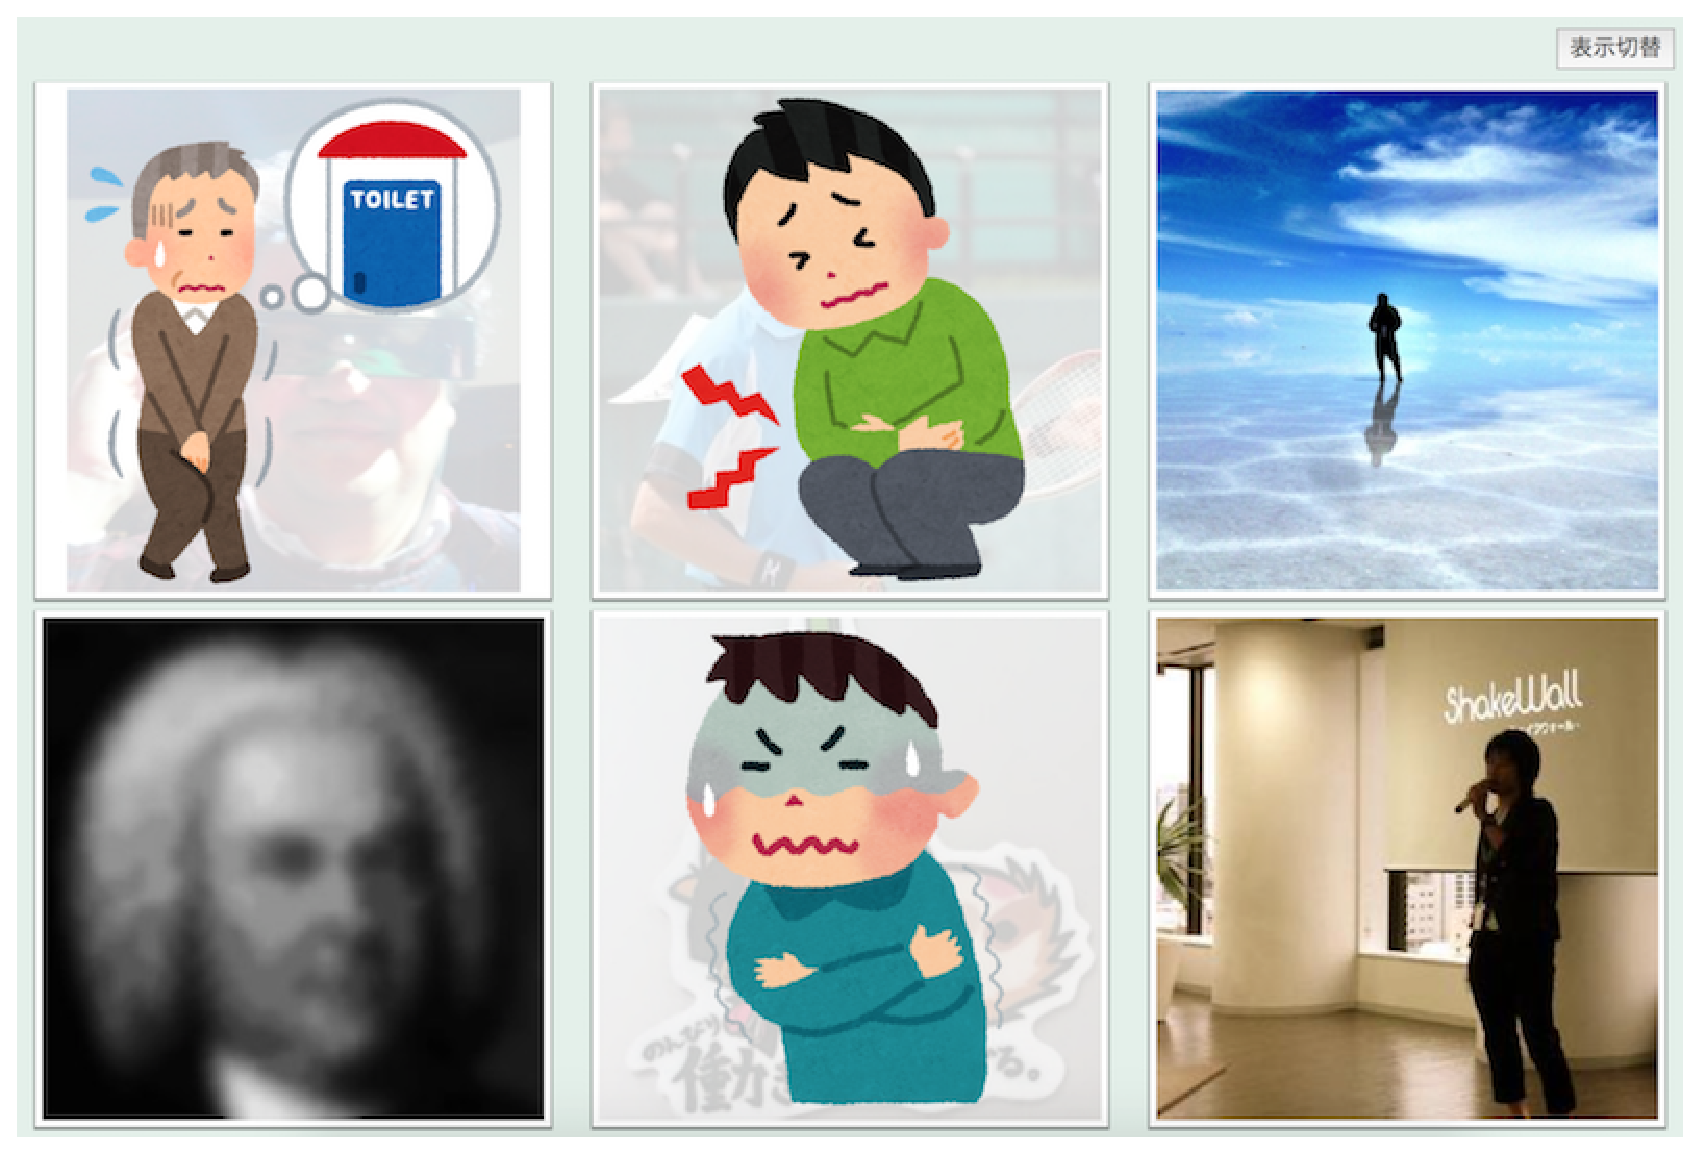
\includegraphics[width=7cm]{images/rescue.eps}
\caption{言い出しにくいことを伝える}
\label{rescue}
\end{figure}

\subsubsection{センサ情報等の表示}

図\ref{sensors}は、明るさ、ドアが最後に開いた時間、気温、風速、天気、メール未読件数、株価、電力使用量を表示した例である。
センサの値やインターネット上の情報、コンピュータの情報などをひと目で把握することができる。

\begin{figure}[h]
\centering
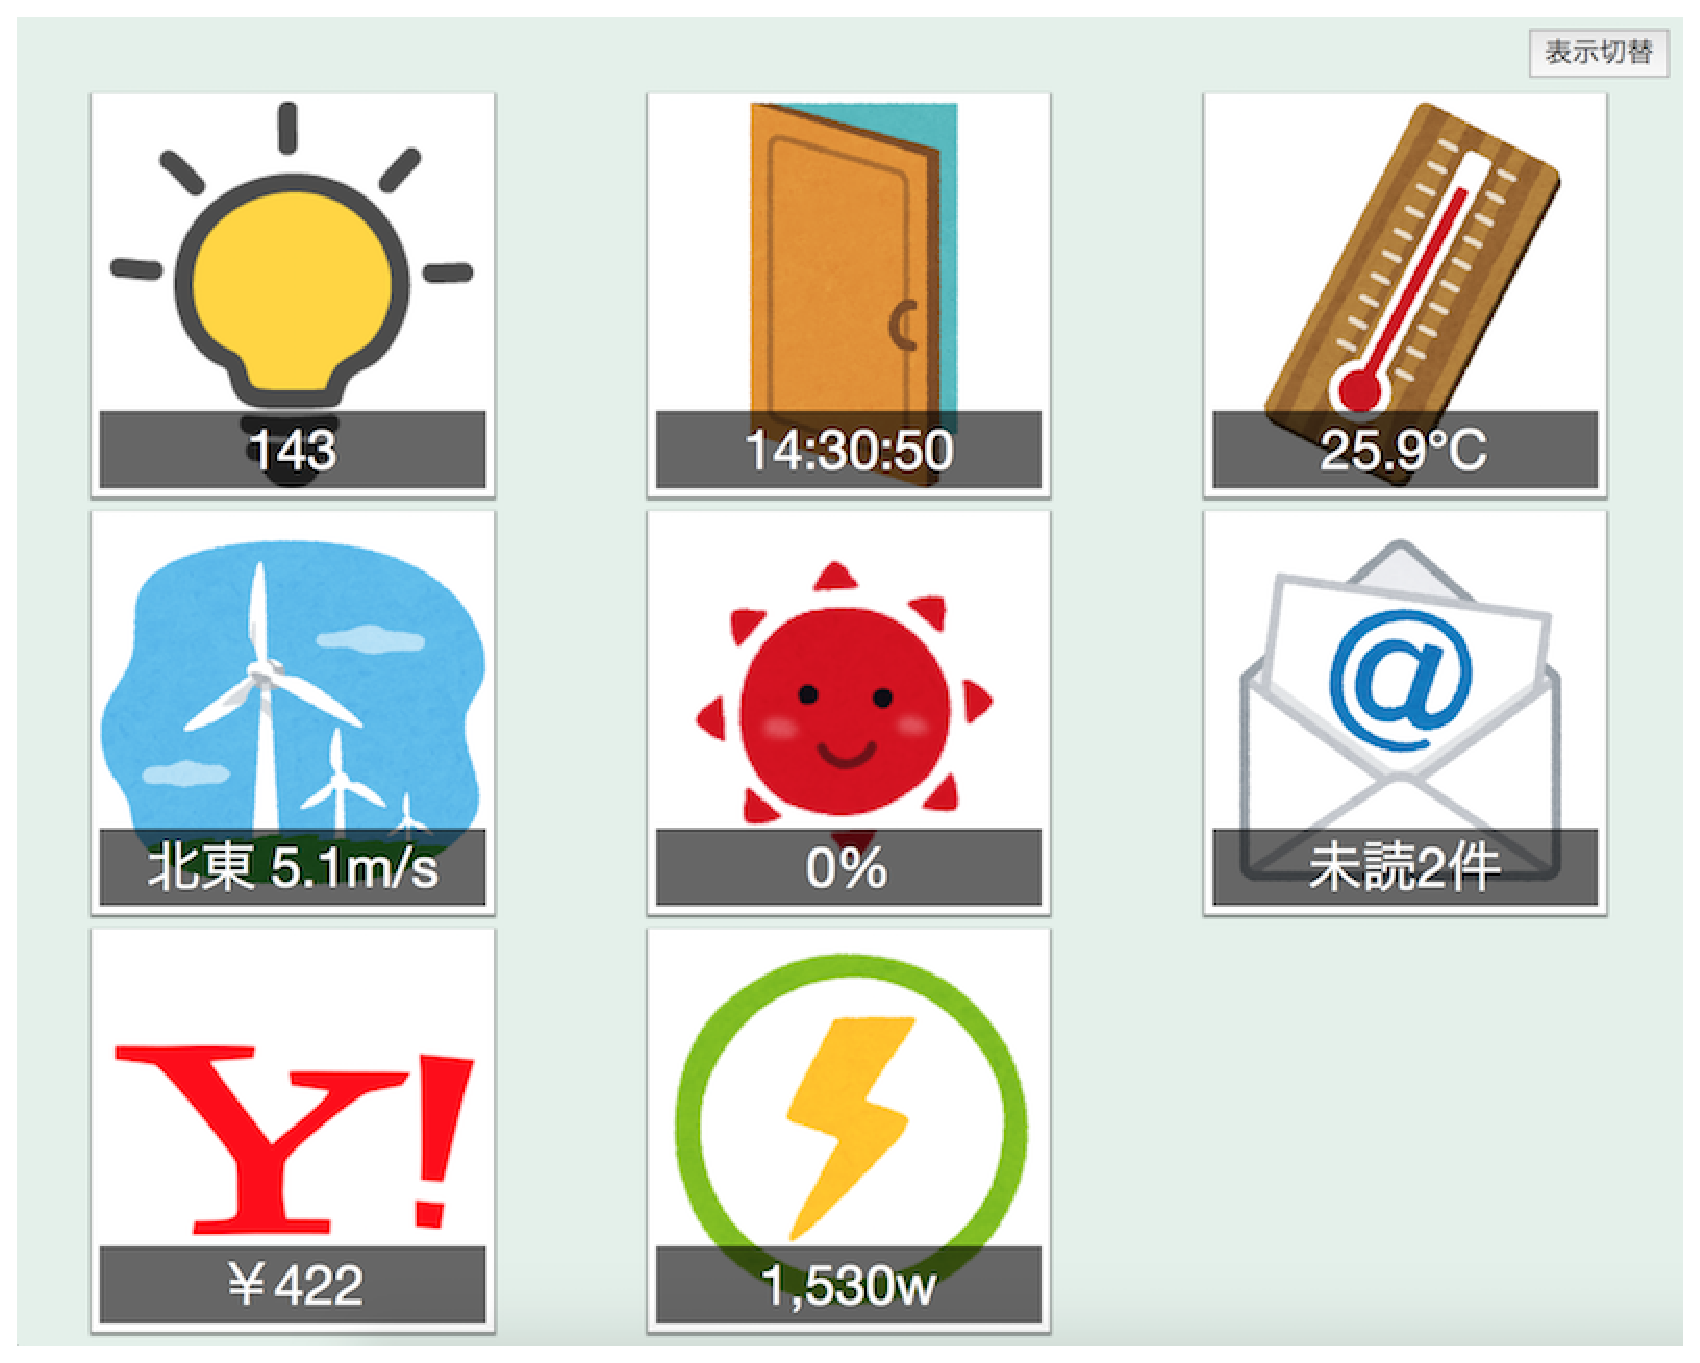
\includegraphics[width=7cm]{images/sensors.eps}
\caption{センサやWebの情報を表示}
\label{sensors}
\end{figure}

\subsubsection{家庭内サイネージ}

図\ref{home}は家庭での利用例である。
左上の夕食は家で食べるかという問いかけに対し、短いメッセージでを送ったり画像で返答することもできる。
また、ペットなど人間以外にセンサを取り付けて投稿させることも可能である。

\begin{figure}[h]
\centering
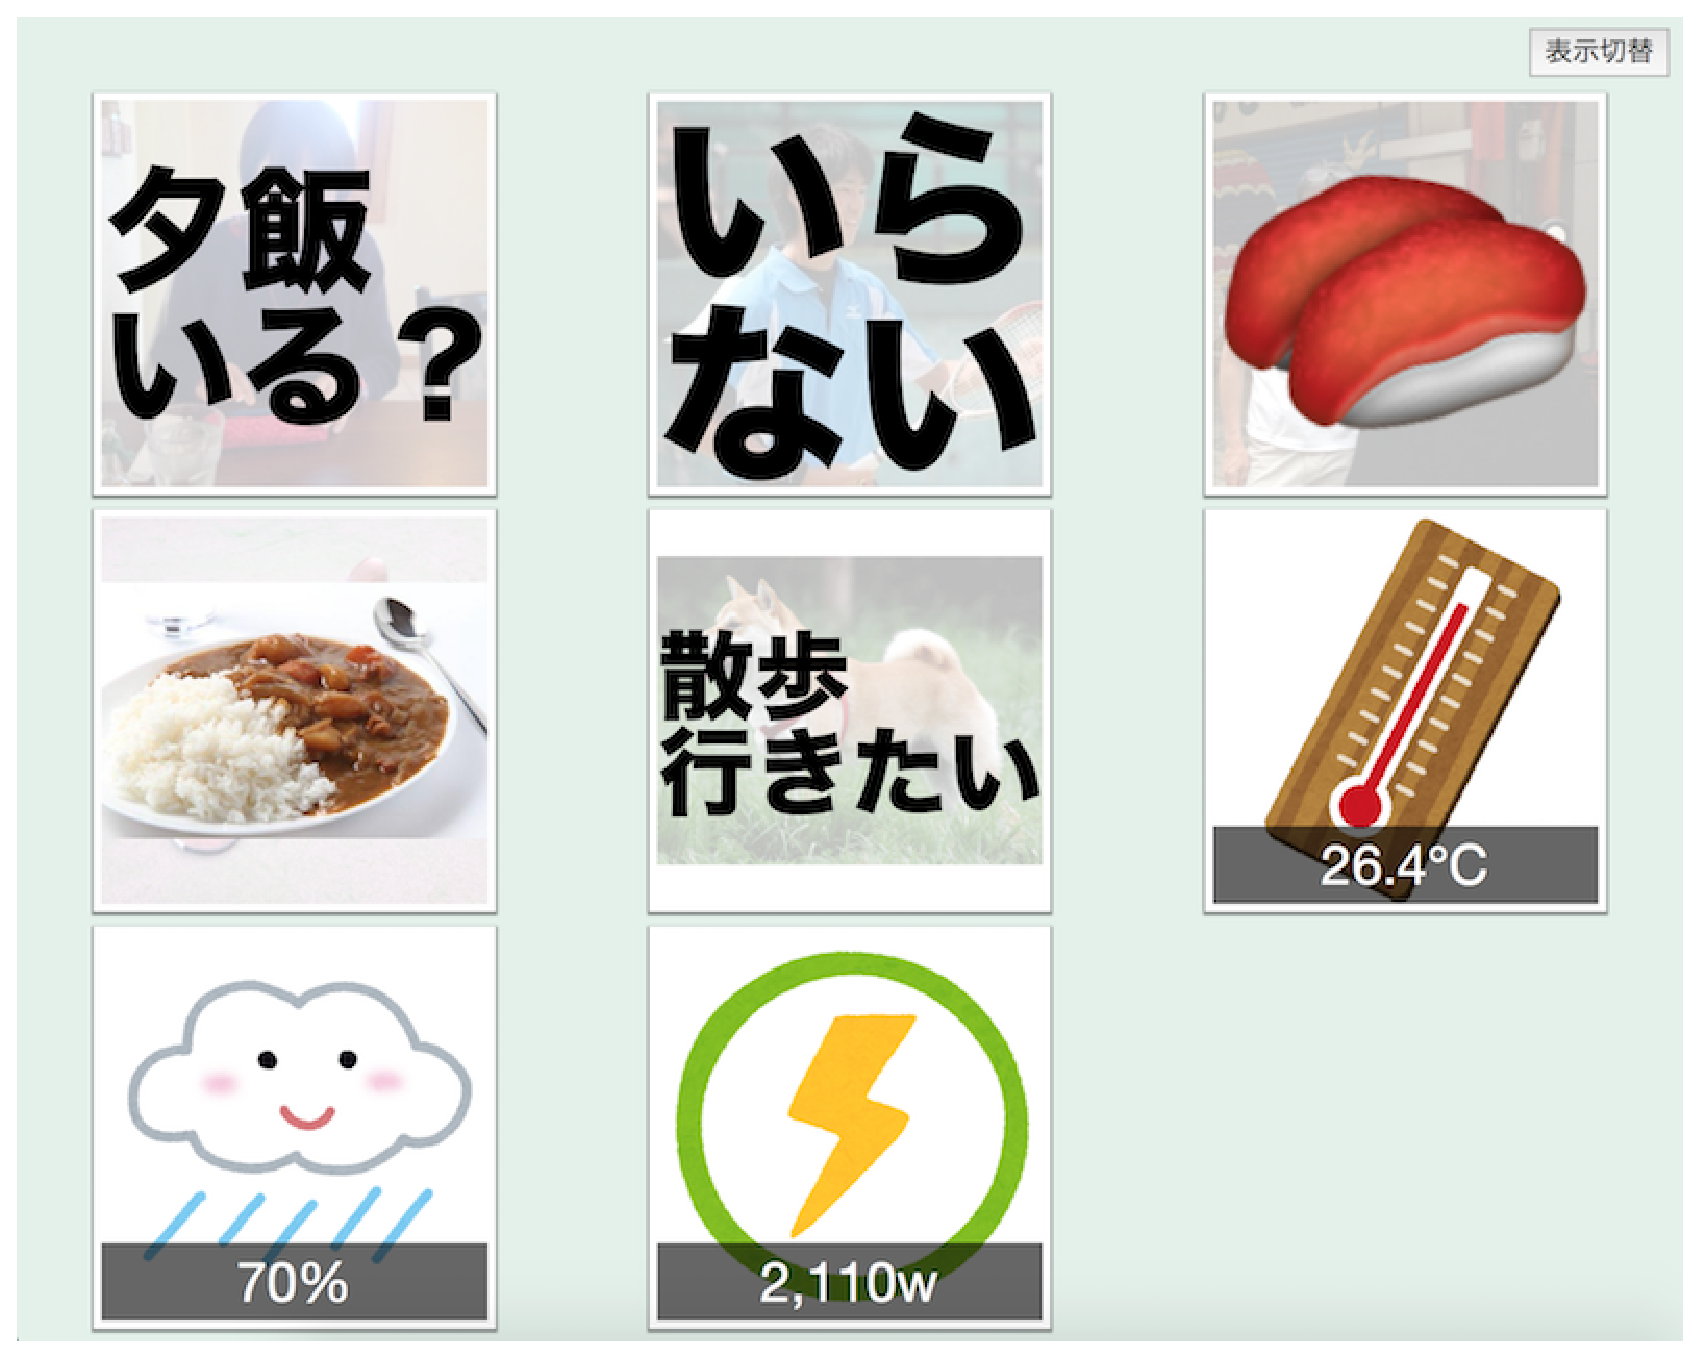
\includegraphics[width=7cm]{images/home.eps}
\caption{家庭での利用}
\label{home}
\end{figure}
\section{実装}

本章ではわかるらんどの実装について述べる。

クライアントはブラウザ上のJavaScriptで実装した。

サーバーは並列計算プリミティブLindaをWebサーバ上に実装したlinda-serverを用いて実装している。
Lindaとは1980年代に生まれた並列処理を行うための実装モデルで、
タプルスペース(tuplespace)と呼ばれる共有メモリ空間にデータレコード(タプル)を格納する。
linda-serverを使用することで、各クライアントやデバイス間で直接送信をする処理を記述する必要が無く、
非常に簡潔に拡張性の高い並列処理環境を実現できる。

わかるらんどへの入力はHTTP通信が可能な環境であれば可能であるため、各種の入力ハードウェアを作ることができる。
図\ref{button}は「へぇ〜」というスタンプを表示する入力装置である。図\ref{10key}は外付けのテンキーのキーに各種のスタンプの入力を割り当てたものである。
このようにブラウザの投稿画面だけでなく、現状のGUIでは利用されないようなデバイスを作ってわかるらんどの入力装置として利用することができる。

\begin{figure}[h]
\centering
\includegraphics[width=7cm]{images/button.eps}
\caption{「へぇ〜」専用入力装置}
\label{button}
\end{figure}

\begin{figure}[h]
\centering
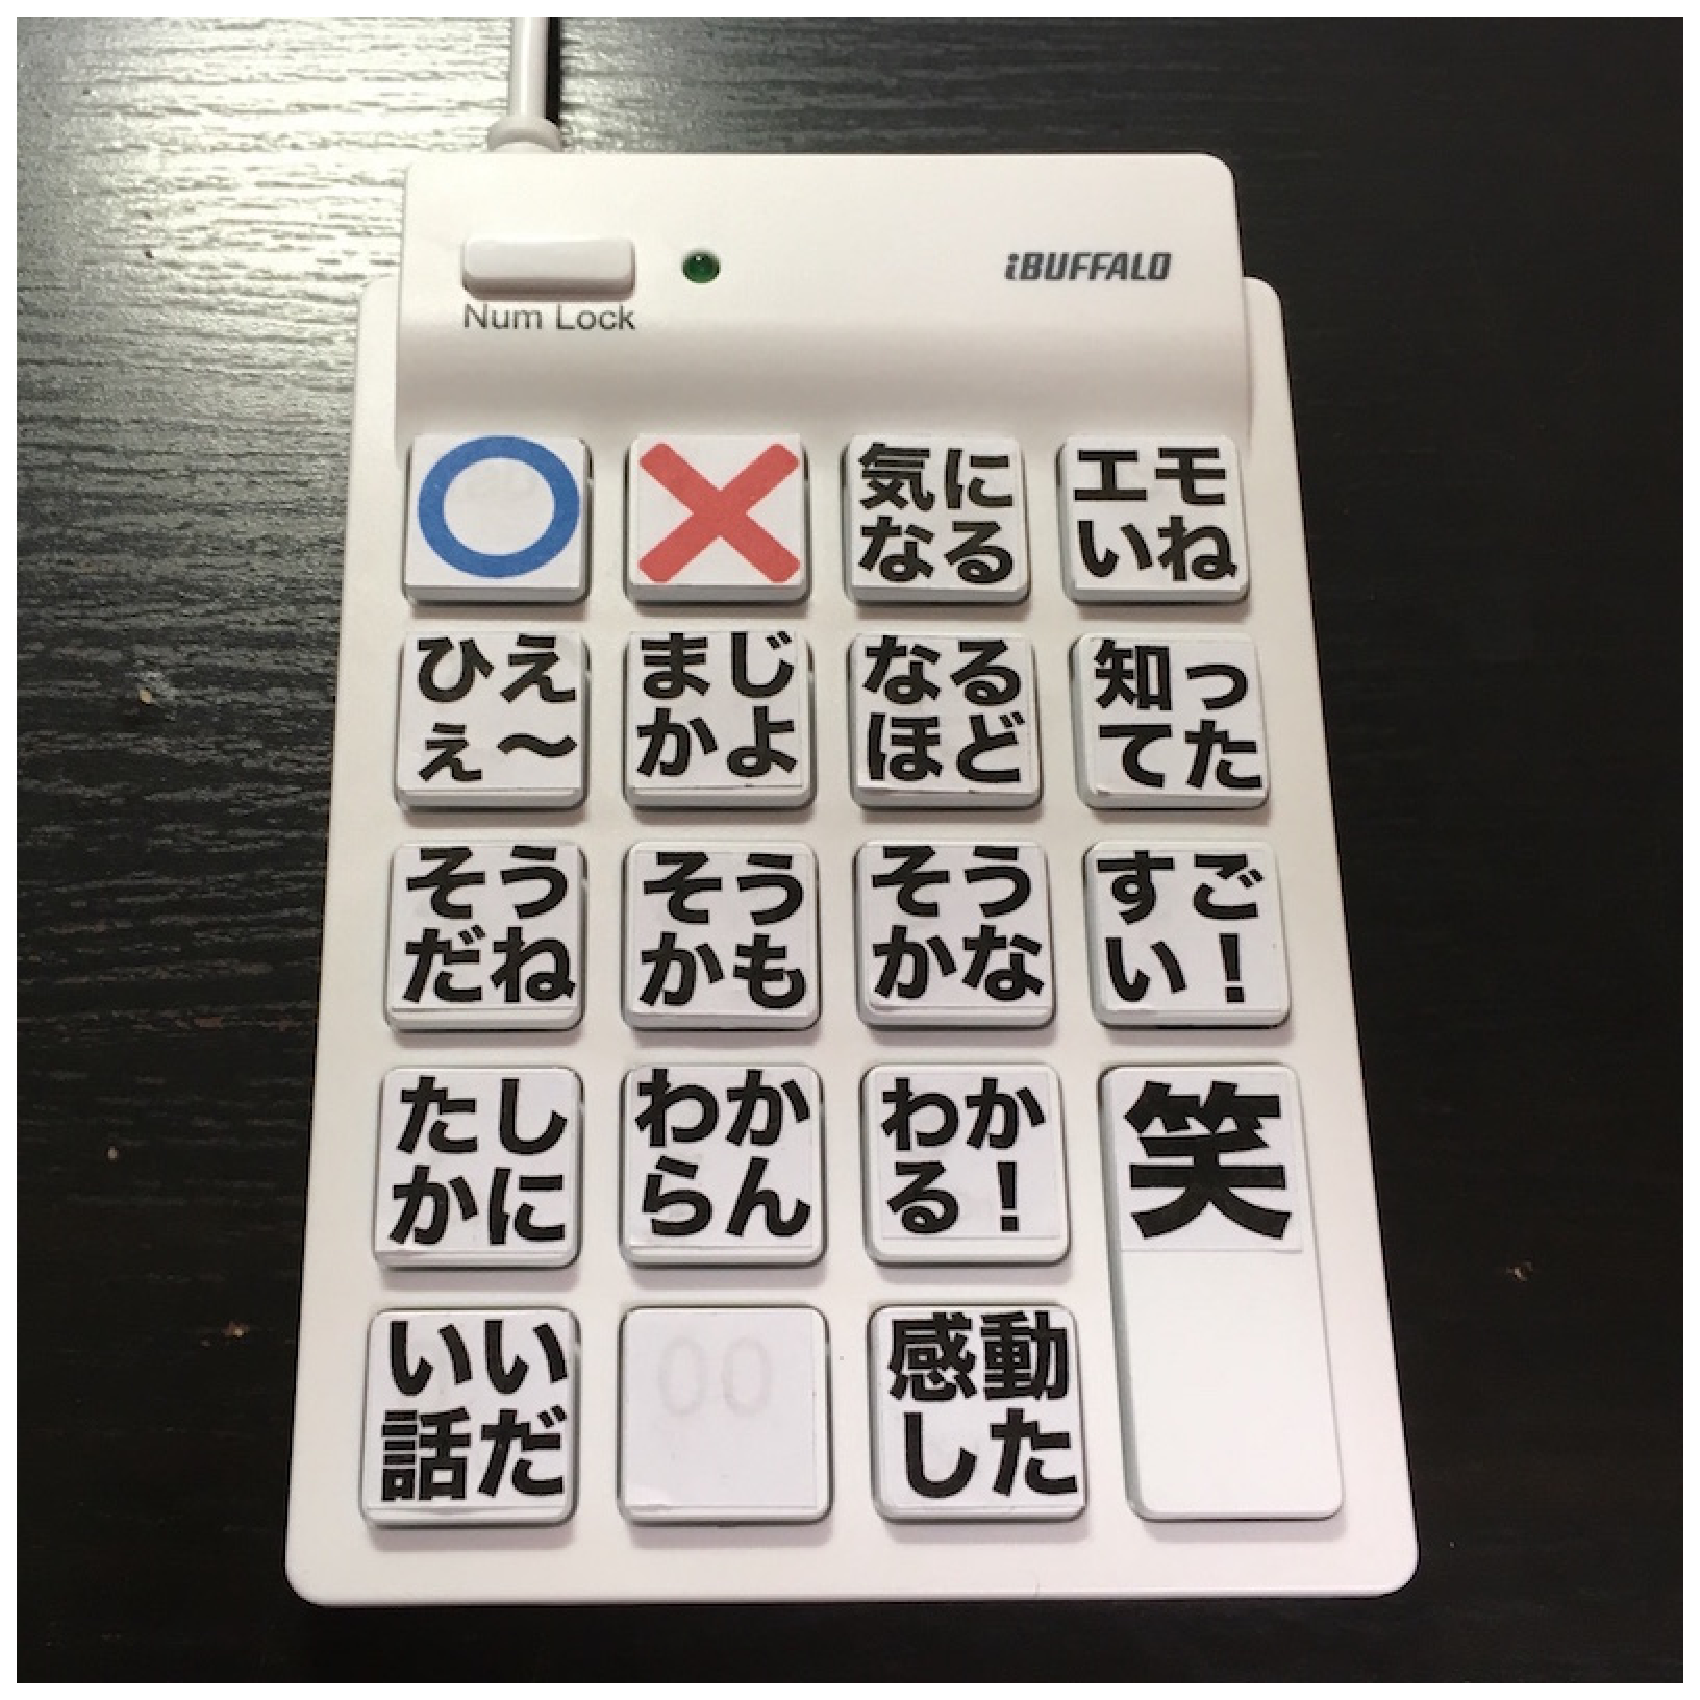
\includegraphics[width=7cm]{images/10key.eps}
\caption{テンキーを利用した入力装置}
\label{10key}
\end{figure}
\section{議論}
近年,学会などでタイムライン表示のテキストチャットが
利用される機会が増えている\cite{wiss_challenge}が、
WISS2009の実証実験\cite{nishida2011}によれば,
全参加者の半分弱しかログインして1回以上発言していなかった.
またWISS2015では,252アカウントが1回以上発言し総発言数は2,948回であったが,
図\ref{powerlaw}のようにアカウントと発言数は冪分布になっており,
発言数上位20\%の50アカウントによる発言が総発言数の78.1\%にあたる2,305回を占めていて,
特定の人ばかりが発言して,発言しない人は全く発言しない傾向が顕著に現れた.

\begin{figure}[h]
\centering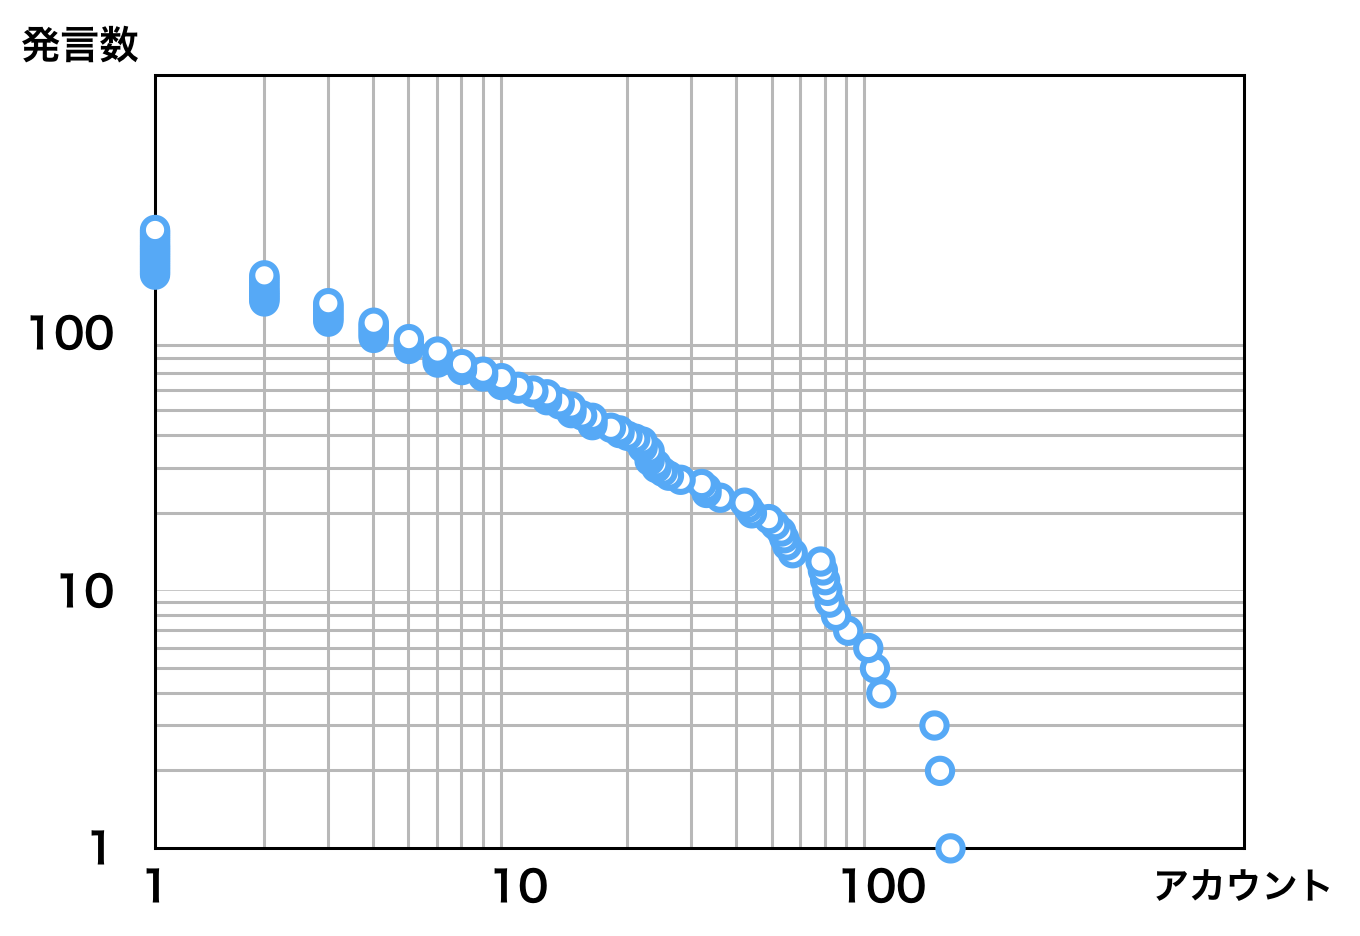
\includegraphics[width=7cm]{images/powerlaw.png}
\caption{WISS2015のチャットのアカウントと発言数の分布の両対数グラフ}
\label{powerlaw}
\end{figure}

『わかるらんど』は長文の高度な発言は期待しておらず,
「なるほど」「わからん」「笑」などといった相槌のようなものを
視覚化してひと目で把握できるようになることを期待している.
本当は議論に参加したいけど声が出ない/手を上げる勇気がない人でも
「なるほど」「わかる」などを『わかるらんど』に投稿することで「参加」することができる.
\section{むすび}

このサンプルは次の環境を用いて動作を確認した.
\begin{itemize}
\item UNIX用の p\LaTeXe (p\TeX3.1.2)
\item Windows用の p\LaTeXe (p\TeX3.1.3)
\end{itemize}
本スタイルシートが著者諸氏の論文作成に役立つことを期待する.
\section{今後の課題}
今後は,授業やコンファレンスなどで大人数で
『わかるらんど』を利用してもらう実証実験を行うことを考えている.

%%
%%	参考文献
%%
% \begin{thebibliography}{1}

% \bibitem{wiss} WISSホームページ.  http://www.wiss.org/.

% \bibitem{aoki1999} H.~Aoki, B.~Schiele, and A.~Pentland.  Realtime
% Personal Positioning System for Wearable Computers.  In
% \emph{Proceedings of the 3rd IEEE International Symposium on Wearable
% Computers}, pp. 37--43, 1999.

% \bibitem{rekimoto2000} 暦本 純一.  まえがき:WISS2000について.  インタラ
% クティブシステムとソフトウェアVIII, pp. i--ii. 近代科学社, 2000.

% \end{thebibliography}

\balance %最後の高さを揃えるために必要 (2012/9/27:watanabe, Igarashi)
\bibliographystyle{jwiss}
\bibliography{wiss_template}

%%%%%%%%%%%%%%%%%%%%%%%%%%%%%%%%%%%%%%%%%%%%%%%%%%%%%%%%%%%%%%%%%%%%%
%%%%%%%%%%%%%%%%%%%%%%%%%%%%%%%%%%%%%%%%%%%%%%%%%%%%%%%%%%%%%%%%%%%%%
%% WISS2012では,「未来ビジョン」は以下のように,本文と同様の2段組形式で記載する.
%% 図を用いても良いが,枠のサイズ(縦93mm)を変更してはならない.
%% (WISS2010では,縦118mmでしたのでご注意下さい)

\begin{figure*}[!b]
\setlength{\unitlength}{1mm}\fboxrule=0.5pt

\vspace{-93mm} %% 未来ビジョンの枠が下がってしまうのを防ぐ WIS2012 カメラレディテンプレで追加  (2012/9/27:watanabe, Igarashi)

% 未来ビジョンの枠の描画
\begin{center}
\framebox[0.95\textwidth]{
\begin{minipage}{0mm}\begin{picture}(0,91)(0,0)\end{picture}\end{minipage}
}
\end{center}
\vspace*{-93mm}	% 未来ビジョンの枠の縦幅分だけ戻す

% 未来ビジョンの内容
\newbox\FUTURE
\setbox\FUTURE=\vbox{
\begin{minipage}[b]{0.9\textwidth}
\begin{multicols}{2}	% 二段組にする
\section*{未来ビジョン}
\setlength{\parindent}{10pt}	% 段落先頭の字下げ

% % % % % % % % % % % % % % % % % % % % % % % % % % % % % %
%	   未来ビジョンは,下記に記入して下さい		  %
% % % % % % % % % % % % % % % % % % % % % % % % % % % % % %

\vspace*{-1mm}

% フォントサイズ指定
\normalsize
%\large
%\small\setlength{\baselineskip}{12pt}
%\footnotesize\setlength{\baselineskip}{12pt}

わかるらんどは「人の気持ちを察したい」という思想から作られたシステムである.
初期のプロトタイプは文字が書かれた札を掲げるというアナログなものだった.
会議やコンファレンスなど多人数に向けての発表の場において最も悲しいことは,聴衆から何のフィードバックもないことである.
「わからん」「なるほど」といった簡単な相づちがあるだけでも印象は異なる.
私自身が口下手で感情のアウトプットが得意なほうではないこともあって,
思ったことを口にしやすいコミュニケーション環境をインタフェースの工夫によって作り上げることがこの研究のミッションである.
わかるらんどが私と同じ悩みを抱えている人の一助になれば幸いである.

%% 文章を補う図表を利用してもよい.
\vspace*{5mm}
\includegraphics[width=0.95\columnwidth]{images/wakaru.eps}
% % % % % % % % % % % % % % % % % % % % % % % % % % % % % %
%	   未来ビジョンは,上記に記入して下さい		  %
% % % % % % % % % % % % % % % % % % % % % % % % % % % % % %

\end{multicols}
\end{minipage}
}

% 未来ビジョンの内容の描画
\newlength{\FUTUREHT}
\setlength{\FUTUREHT}{\the\ht\FUTURE}	% 未来ビジョンの内容の縦幅保存
%\typeout{\the\wd\FUTURE}
%\typeout{\the\ht\FUTURE}
\hspace*{0.045\textwidth}	% 未来ビジョンの内容の横位置調整
\box\FUTURE
%\typeout{\the\FUTUREHT}
\vspace*{-\the\FUTUREHT}	% 未来ビジョンの内容の縦幅分だけ戻す
\vspace*{-10.9mm}		% 微調整

% 未来ビジョンの枠の領域の再確保(これがないと枠が下に沈み込む)
\begin{center}
\fboxrule=0pt
%\fboxrule=2pt	% デバッグ用: コメントアウトをやめて,同じ位置に枠が出るか?
\framebox[0.9\textwidth]{
\begin{minipage}{0mm}\begin{picture}(0,91)(0,0)\end{picture}\end{minipage}
}
\end{center}
\end{figure*}

%%%%%%%%%%%%%%%%%%%%%%%%%%%%%%%%%%%%%%%%%%%%%%%%%%%%%%%%%%%%%%%%%%%%%
%%%%%%%%%%%%%%%%%%%%%%%%%%%%%%%%%%%%%%%%%%%%%%%%%%%%%%%%%%%%%%%%%%%%%
\end{document}
